% !TEX root = ../../../Masterthesis.tex

\chapter{Star Trek X: Nemesis}

\section{Remus (Main Title)}\label{sec:st 10}
%-----------------------------------------------------------------------------
% Introduction
%-----------------------------------------------------------------------------
\begin{figure}
\center
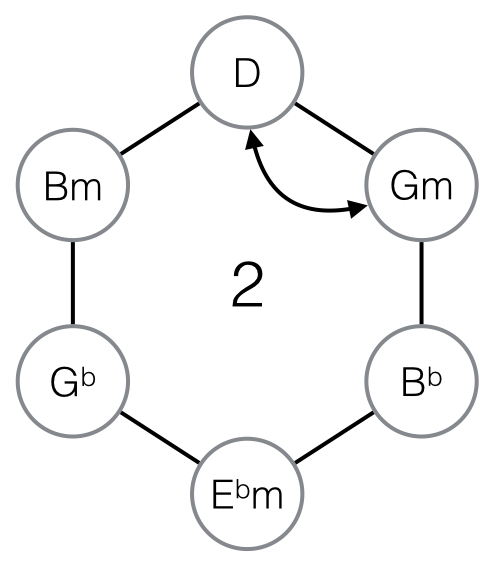
\includegraphics[width=0.5\linewidth]{ST10_main_title_intro_1}
	\caption{ST 10: Main Title Intro 1}
	\label{ST10_main_title_intro_1}
	\setfloatalignment{b}
\end{figure}

\noindent\newthought{The music begins} with the introduction of the Paramount logo. This time there is a synth and string pad slowly evolving through \(\hat{5}-\hat{1}-\hat{5}\) ending on a piercing, sweeping, high-pitch pad over D\(^{\triangle 7}\) (figure \ref{ST10_main_title_intro_1}). This fades down fairly quickly to a D\(^{5}\), which provides the harmonic bed for the melody. The melody starts by ascending two M3's, resting on the fifth, creating an uneasy feeling. The melody uses the fifth mode of melodic minor\footnote{Mixolydian\(\flatx{6}\)=[0,2,4,5,7,8,T]} giving both minor \(iv\) and \(v\). 

%-----------------------------------------------------------------------------
% Introduction part 2
%-----------------------------------------------------------------------------
\begin{figure}
\center
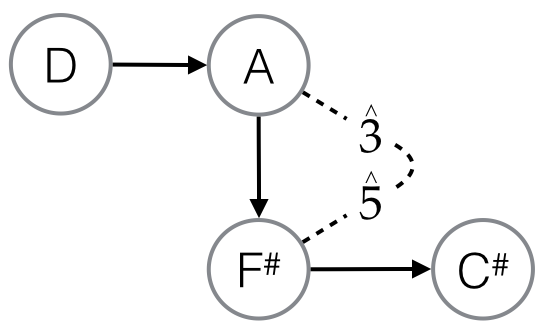
\includegraphics[width=0.5\linewidth]{ST10_main_title_intro_2}
	\caption{ST 10: Main Title Intro 2}
	\label{ST10_main_title_intro_2}
	\setfloatalignment{b}
\end{figure}
In m.10, the famous "Courage" Theme comes to life as the Star Trek tittle hits the screen. It modulates and repeats as the subtitle ``Nemesis'' is revealed. The modulation makes a coupling through the \(\hat{3}\) of A, making it the new \(\hat{5}\) of \fiss (figure \ref{ST10_main_title_intro_2}).

%-----------------------------------------------------------------------------
% A
%-----------------------------------------------------------------------------
\begin{figure}
\center
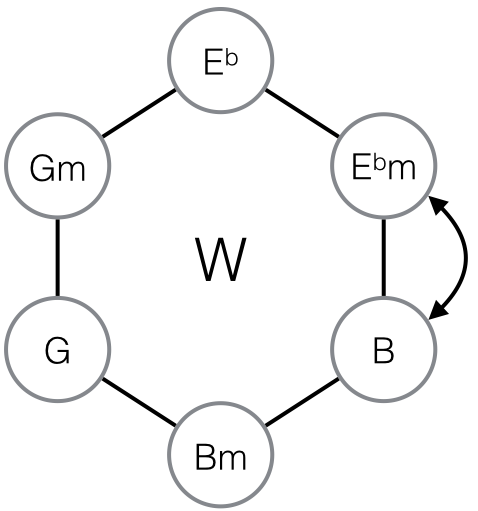
\includegraphics[width=0.5\linewidth]{ST10_main_title_A}
	\caption{ST 10: Main Title A}
	\label{ST10_main_title_A}
	\setfloatalignment{b}
\end{figure}
After a short percussive pattern with military snare drums and timpani, the main theme plays. This happens while we fly toward a number of planets, traveling all the way down to an alien city. Supporting the melody is percussion and a metallic synth, providing an ominous military feeling.The scale is pure minor and the chords alternate between \(vi(I)-IV\) (figure \ref{ST10_main_title_A}).

%-----------------------------------------------------------------------------
% B
%-----------------------------------------------------------------------------
As soon as the dialogue starts, the music drops down and an eerie melody plays. The sonority perceived is that of chords built upon [048]'s, thanks to the same Mixolydian\(\flatx{6}\) used in the introduction. 

%-----------------------------------------------------------------------------
% PDF
%-----------------------------------------------------------------------------
\clearpage
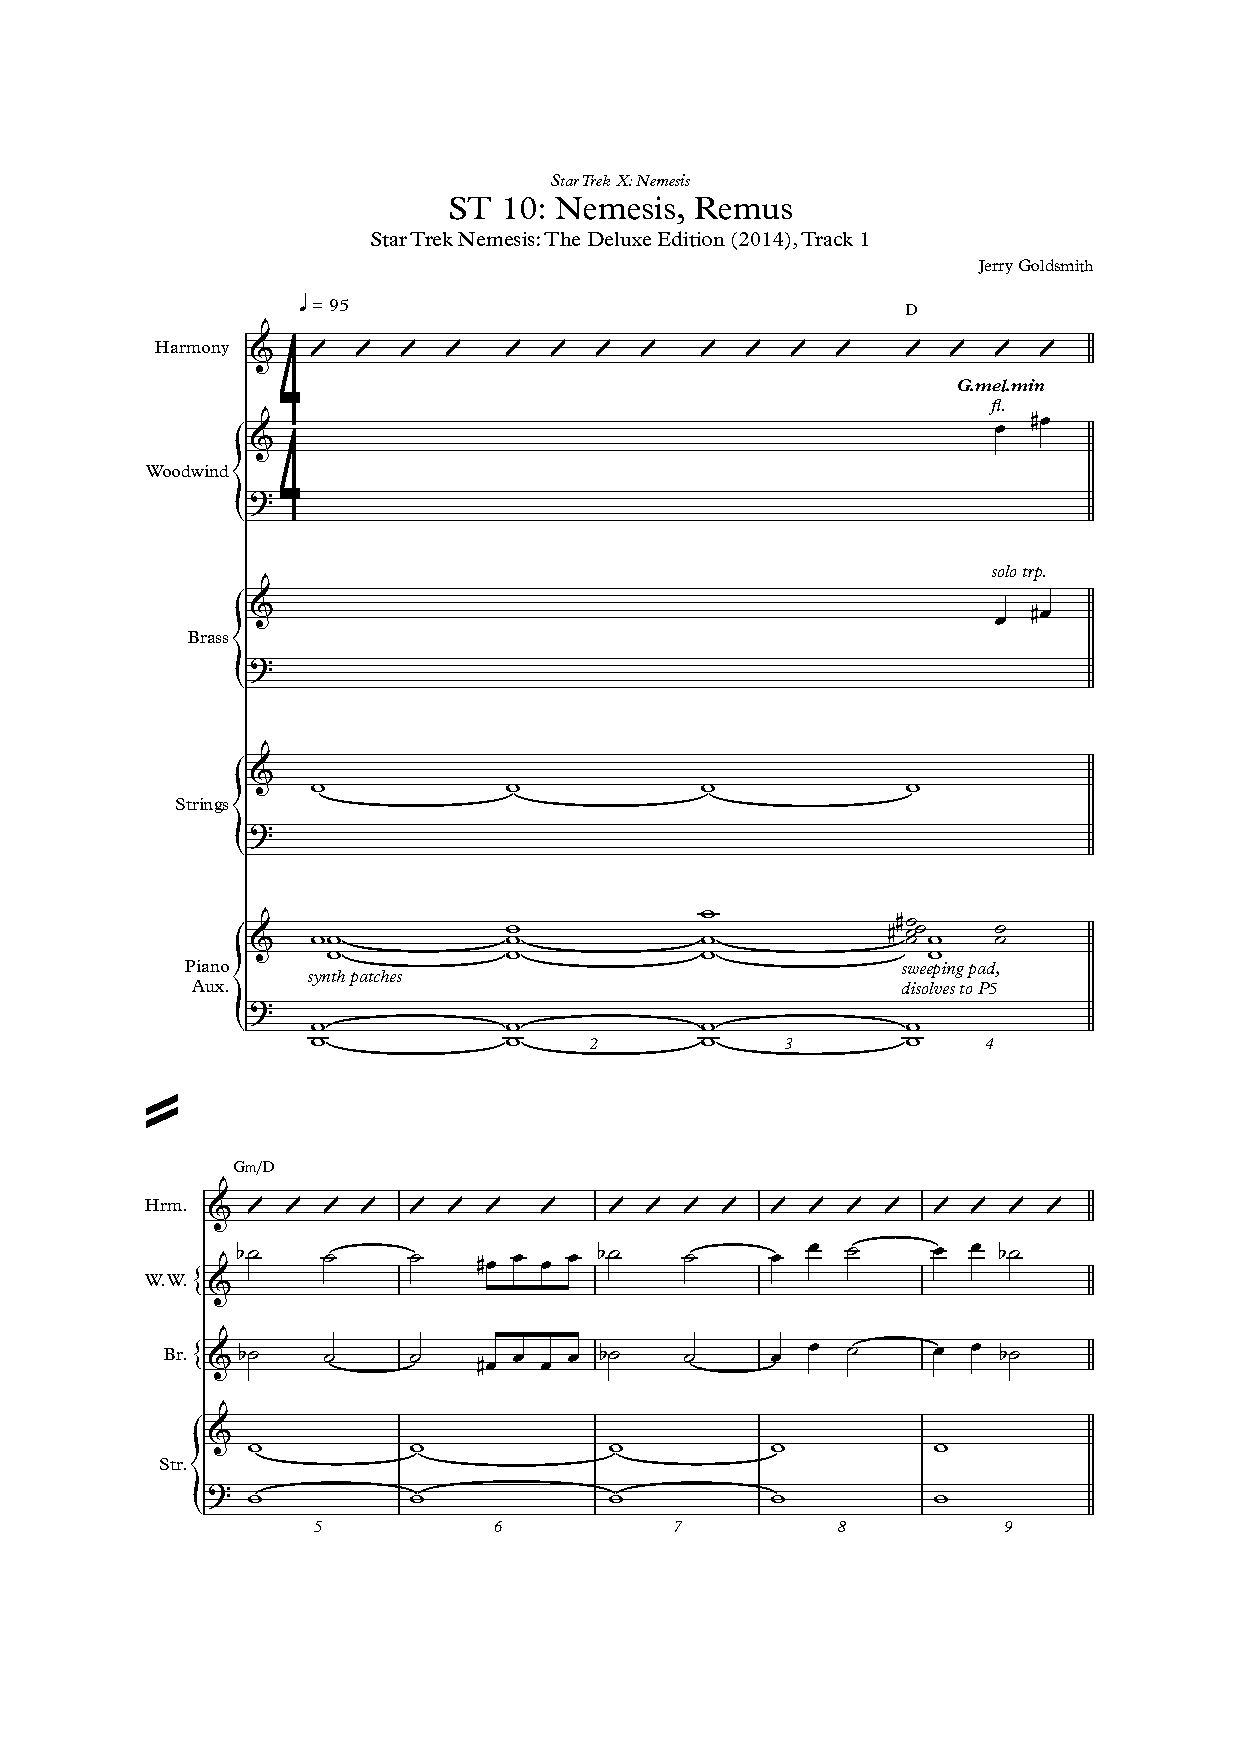
\includepdf[pages=-,pagecommand=\thispagestyle{fancy}]{pdf/ST10/ST10_Remus.pdf}

% Reviewed